\section{Improving the pairing efficiency with SPANet}


\subsection{Choice of the optimal inputs for the training}
As mentioned in section \ref{section: spanet architecture} we can give SPANet global and sequential inputs for the training. The sequential inputs being the ones that can have an arbitrary number of vectors per event, they will correspond to the information of the jets used for the pairing. On the other hand, the global vectors are the ones that will have a single vector per event, so they correspond to event level information.

In order to find the optimal training that maximizes our pairing efficiency, we started by testing different configurations. As precised before, we want 4 jets in the final state, nevertheless due for instance to QCD processes even if in an event there is di-Higgs production decaying into 4 b quarks, we can have more than 4 jets in the final state. Hence, we want to start by checking how much do we gain in signal efficiency by considering other jets in the final state with lower b-tag score for the pairing. This can be seen in table \ref{table:signal_efficiency}. We first present the percentage of signal where the $k^{th}$ jet was matched, meaning that this $k^{th}$ jet was matched to one of the gen jets. We also show the percentage of signal of fully matched events, meaning the events for which 4 jets are matched to the 4 gen jets. Out of the total number of events 92.9\% are fully matched and the percentage of fully matched events when considering the first 4 leading jets is 90.2\%. According to table \ref{table:signal_efficiency}, we can see that most of the remaining signal efficiency is gained by considering a fifth jet for the paring (we gain 2.5\% out of 2.7\%). 

From these results, we conclude that the highest signal efficiency is obtained by considering either 4 or 5 jets for the pairing. Therefore, we will train SPANet using 4 and 5 jets as sequential inputs. We will also make one test considering 6 jets as sequential inputs, nevertheless this did not increase our performance, hence the choice of stopping at 5 jets for the pairing.


\begin{table}[h!]
\centering
\begin{tabular}{|p{1cm}||p{6cm}||p{6cm}|}
 \hline
 k  & Percentage of the signal with the $k^{th}$ jets matched & Percentage of signal fully matched events with the $k^{th}$ jet matched\\
 \hline
 4 &  ? & 90.2\\
 5 & 2.76 & 2.52 \\
 6 & 0.27 & 0.25 \\
 $\geq$7 &  $\approx$0.03 &  $\approx$0.02 \\
 \hline
\end{tabular}
\caption{Signal Efficiency}
\label{table:signal_efficiency}
\end{table}

For the first SPANet trainings, we will compare the performance of using either 4 or 5 jets as sequential inputs. We will use as first figure of merit for the performance the inclusive pairing efficiency and the \textit{total} pairing efficiency. We define the pairing efficiency as:

\begin{equation*}
    \text{Pairing efficiency}=\frac{\text{Correctly fully matched events}}{\text{Total number of fully matched events}}
\end{equation*}

However, as we explained earlier, the number of fully matched events is larger when considering a fifth jet for the pairing, hence to have a fair comparison between the trainings we need to compute the \textit{total} pairing efficiency which is given by:
\vspace{-0.2cm}
\begin{eqnarray*}
\text{Total efficiency} & = & \text{Pairing efficiency} \times \text{Fraction of fully matched events} \\
% & = & \frac{\text{Correctly fully matched events}}{\text{Total number of fully matched events}} \times \frac{\text{Total number of fully matched events}}{\text{Total number of events}} \\
& = &\frac{\text{Correctly fully matched events}}{\text{Total number of events}}     
\end{eqnarray*}

This is why in table \ref{table: First comparison} we summarize these first results by showing the configuration of the training as well as the pairing efficiency and for a fair comparison, the total pairing efficiency.

\begin{table}[h!]
\centering
\begin{tabular}{|M{2cm}|M{5cm}|M{2cm}|M{2cm}|M{2cm}|}
 \hline
 Training  & Configuration &  Pairing efficiency & Fraction of fully matched events & Total pairing efficiency \\
 \hline
 4 jets &  \raggedright 4 jets considered for the pairing and using \begin{itemize}[itemsep=0.01em]
    \item \pt
    \item $\eta$
    \item $\phi$
    \item b-tag
 \end{itemize} 
 as kinemtic information & 0.984 & 0.901 & 0.887 \\
 \hline
 4 jets 5 global & \raggedright 4 jets considered for the pairing and a 5$^{\text{th}}$ given as global information. We use \begin{itemize}[itemsep=0.01em]
    \item \pt
    \item $\eta$
    \item $\phi$
    \item b-tag
 \end{itemize} 
 as kinematic information  & 0.984 & 0.901 & 0.887\\
 \hline
  5 jets & \raggedright 5 jets considered for the pairing and using \begin{itemize}[itemsep=0.01em]
    \item \pt
    \item $\eta$
    \item $\phi$
    \item b-tag
 \end{itemize} 
 as kinematic information &  0.942 & 0.926 &  0.872 \\
 \hline
\end{tabular}
\caption{Comparison of the efficiency of the first trainings}
\label{table: First comparison}
\end{table}

As explained in the beginning, the global variables only add event level information, therefore in the training using 4 jets 5 global, the fifth jet adds information of kinematics of the system but is not used for the pairing.

From the results shown in Table \ref{table: First comparison}, we can at first say that using this configuration of the trainings, using 4 jets and 5$^{\text{th}}$ global or 4 jets as inputs are more performing. Nevertheless, by considering a 5$^{\text{th}}$ jet as either a global input or for the pairing can help the network as it has more information about the event, therefore, before stopping the trainings using 5 jets, we will try different configurations using 4 jets with a 5$^{\text{th}}$ global and 5 jets as inputs.


In Tables \ref{table:5 jets trainings} and  \ref{table:4 jets trainings}, we show the different configurations for the new trainings as well as their performance. In the new configurations we either vary the kinematical information of the jets or some of the hyperparameters of the model. In the first trainings presented earlier we used what we will call the \textit{Large model}, that uses the default SPANet hyperparameters. However, we wanted to try some of the hyperparameters shown in \textbf{cite}, and this configuration will correspond to the \textit{Lite Model}. The comparison of these models is shown in Table \ref{table:comparison_models}.

\begin{table}[h!]
    \centering
     \begin{tabular}{|c||c|c|}
      \hline
         & Large model &  Lite model\\ 
      \hline
      Hidden dimensions & 64 &  32\\ 
      \hline
      Transformer dimension& 64 & 64 \\ 
      \hline
      Embedding layers & 10 & 8 \\ 
      \hline
      Encoder layers & 6 & 6 \\ 
      \hline
      Trainable parameters & \textbf{2.2 M} & \textbf{0.5M} \\ 
      \hline
      Learning rate & 0.0015 & 0.00659 \\ 
      \hline
      Batch size & 2048 & 2048 \\ 
      \hline
      Optimizer & AdamW & AdamW \\ 
      \hline
      Number of epochs & 50 & 50 \\
      \hline
    \end{tabular}
    \caption{Comparison of Large and Lite Models}
    \label{table:comparison_models}
\end{table}


\begin{table}[h!]
\centering
\begin{tabular}{|M{2.5cm}|M{5.25cm}|M{1.75cm}|M{1.75cm}|M{1.75cm}|}
 \hline
 Training  & Configuration &  Pairing efficiency  & Fraction of fully matched events & Total pairing efficiency \\
 \hline
 5 jets & \raggedright \footnotesize \begin{itemize}[itemsep=0.001em]
    \item \pt
    \item $\eta$
    \item $\phi$
    \item b-tag
    \item Large model
 \end{itemize} & 0.942 & 0.926 & 0.872 \\
 \hline
 5 jets with b-tag preselection \pt regressed & \raggedright  \footnotesize \begin{itemize}[itemsep=0.001em]
    \item \pt
    \item $\eta$
    \item $\phi$
    \item b-tag
    \item Large model
    \item Fifth jet has a b-tag above the medium working point
 \end{itemize}  & 0.975 & 0.913 & 0.890 \\
 \hline
  5 jets \pt regressed and Lite model & \raggedright \footnotesize \begin{itemize}[itemsep=0.001em]
    \item \pt regressed
    \item $\eta$
    \item $\phi$
    \item b-tag
    \item Lite model
 \end{itemize} &  0.969 & 0.926 & 0.897\\
 \hline
 5 jets \pt regressed, Lite model and b-tag preselection & \raggedright \footnotesize \begin{itemize}[itemsep=0.001em]
    \item \pt
    \item $\eta$
    \item $\phi$
    \item b-tag
    \item Lite model
    \item Fifth jet has a b-tag above the medium working point
 \end{itemize} 
  & 0.977 & 0.913 & 0.892\\
 \hline
\end{tabular}
\caption{Different configurations for trainings with 5 jets as sequential inputs}
\label{table:5 jets trainings}
\end{table}

\begin{table}[h!]
\centering
\begin{tabular}{|M{2.5cm}|M{5.25cm}|M{1.75cm}|M{1.75cm}|M{1.75cm}|}
 \hline
 Training  & Configuration &  Pairing efficiency  & Fraction of fully matched events & Total pairing efficiency \\
 \hline
 4 jets 5 global & \raggedright \footnotesize \begin{itemize}[itemsep=0.001em]
    \item \pt
    \item $\eta$
    \item $\phi$
    \item b-tag
    \item Large model
 \end{itemize} & 0.984 & 0.901 & 0.887 \\
 \hline
 4 jets 5 global \pt regressed & \raggedright  \footnotesize \begin{itemize}[itemsep=0.001em]
    \item \pt regressed
    \item $\eta$
    \item $\phi$
    \item b-tag
    \item Large model
 \end{itemize}  & 0.985 & 0.901 & 0.887 \\
 \hline
  4 jets 5 global \pt regressed and Lite model & \raggedright \footnotesize \begin{itemize}[itemsep=0.001em]
    \item \pt regressed
    \item $\eta$
    \item $\phi$
    \item b-tag
    \item Lite model
 \end{itemize} &  0.986 & 0.901 & 0.888\\
 \hline
 4 jets 5 global Lite model & \raggedright \footnotesize \begin{itemize}[itemsep=0.001em]
    \item \pt
    \item $\eta$
    \item $\phi$
    \item b-tag
    \item Lite model
 \end{itemize}  & 0.983 & 0.901 & 0.886 \\
 \hline
 4 jets 5 global with b-tag preselection & \raggedright \footnotesize \begin{itemize}[itemsep=0.001em]
    \item \pt
    \item $\eta$
    \item $\phi$
    \item b-tag
    \item Large model
    \item Fifth jet given as global input has a b-tag above the medium working point
 \end{itemize} 
  & 0.984 & 0.901 & 0.886\\
 \hline
\end{tabular}
\caption{Different configurations for trainings with 4 jets as sequential inputs}
\label{table:4 jets trainings}
\end{table}

From Tables  \ref{table:5 jets trainings} and  \ref{table:4 jets trainings}, we can see that for both either 5 jets or 4 jets 5 global, the best performance is obtained by using \pt reg and the Lite model. However here we only compare the total pairing efficiencies inclusively, but it is also possible to plot them differential as a function of $m_{HH}$, as can bee seen in Figures \textbf{bla, bla}. In Figure \textbf{bka} we can see that using different configurations for 4 jets and 5th global does not make impact much our total pairing efficiency. On the contrary, in Figure wee can see how much difference it makes to change the configuration of the training.

The next step is to compare these two models to the performance of the $D_{HH}$-method presented in section \ref{section: HH4b}. The comparison is done for events for which we have $\Delta D_{HH} > 30$ GeV, as we only could implement this method for these events. In Figure \textbf{bla} we show how these 2 models outperform the $D_{HH}$-method. 

\vspace{0.2cm}

\noindent In conclusion, we obtained 2 models:

\begin{itemize} [itemsep=0.1em]
    \item 4 jets as sequential inputs with a 5th global jet using the \pt reg $\eta, \phi$ and btag of the jets as well as the lite model
    \item 5 jets as sequential inputs using the \pt reg $\eta, \phi$ and btag of the jets as well as the lite model
\end{itemize}

\noindent which have the highest total efficiency and that outperform the pairing efficiency used in the $D_{HH}$-method.

We also tried to asses the performance of these trainings evaluated on datasets where we only have 4 jets, but these evaluations are not correct due to the difference of phase space between the train and the test files. Moreover, we performed a test by training without the b-tag of the jet as input, nevertheless the performance was much worse than by including it in the inputs.

Even though the training using 5 jets as inputs outperforms the training using 4 jets with a 5$^{\text{th}}$ global, as a next figure of merit to choose our optimal model, it is important to verify if when applying our model in data, we observe background mass sculpting.

\newpage

\subsection{Background mass sculpting}
In addition to the pairing efficiency, another figure of merit we use in order to select the best model is the mass sculpting of the background. This is a very important feature as if we evaluate our model in a sample with mostly background events, we should not observe a fake peak of events around the signal region. 

To verify this, we will use the models we presented in the last section and evaluate them in a sample of 2b data. This dataset contains data collected in 2022 during the Run 3, and as explained in section \ref{subsection:cutflows} due to the requirements of the 2b region, we have mostly background events and the signal contribution due to mistagging of the jets is negligible. Hence, if we evaluate our model here, we should not observe a peak of events in the $m_{HH}$ plane around the signal region (defined in section \ref{section: HH4b}). Indeed, in Figure \textbf{bla}, we show the 2D mass distribution of the evaluation of our model on signal events. We can see that most of the predicted events are in the signal region, as we would expect. Contrary, in Figure \textbf{bla}, we show the 2D mass distribution of the evaluation of our model on 2b data. We can see that there is not a peak of events in the signal region, which is indeed what we expected. 


For more clarity, we can compare these distributions in the 1D plane. These are shown in Figures \textbf{bla bla} for the leading and the subleading Higgs respectively. In these plots we can compare the two models more accurately and conclude that there is less sculpting when considering the training with 5 jets, for both the leading and the subleading Higgs. Therefore, the model where we give 5 jets as inputs, with \pt ref and using the lite hyperparameters not only has the best pairing efficiency but also the mass sculpting is smaller than with the 4 jets model. Therefore, in the following sections, we will use this model.

The next question that arises when performing these tests, is that after performing several trainings with 5 jets, we observed a variability in the results, which is why, we decided to delve onto the variability of these trainings.

\subsection{Studies for the training variability}
So as to asses the variability of our model, we performed several trainings fixing the seed to randomly initialize the weights. As a first test to adress this variability issue, in addition to fixing the weights, we started by verifying if the Pytorch version used for the training had an impact on the variability. To do so, we performed 3 different trainings fixing the seeds to 0, 1 and 2 for 3 different versions of Pytorch. We concluded that the variability is independent of the version we use when we fix the seed to initialize the weights, so we decided to use the latest version (2.2.2) for our future trainings. Then, using this version we performed 26 different trainings with 26 different seeds to observe the variability. The results are shown in Figure \ref{fig: 5j variability}, where we plot the validation accuracy for each training. We can see that it clusters around 2 different values: 96.6\% and 94.5\%. Around each value we have a spread of around 0.3\%. Therefore, with these results we can indeed state that there is a large variability of our model (~2\%), with which we don't outperform the pairing efficiency of Run 2. To solve this this, we aim to modify our hyperparameters in order to stabilize our model.

\begin{figure}[hbt]
    \centering
    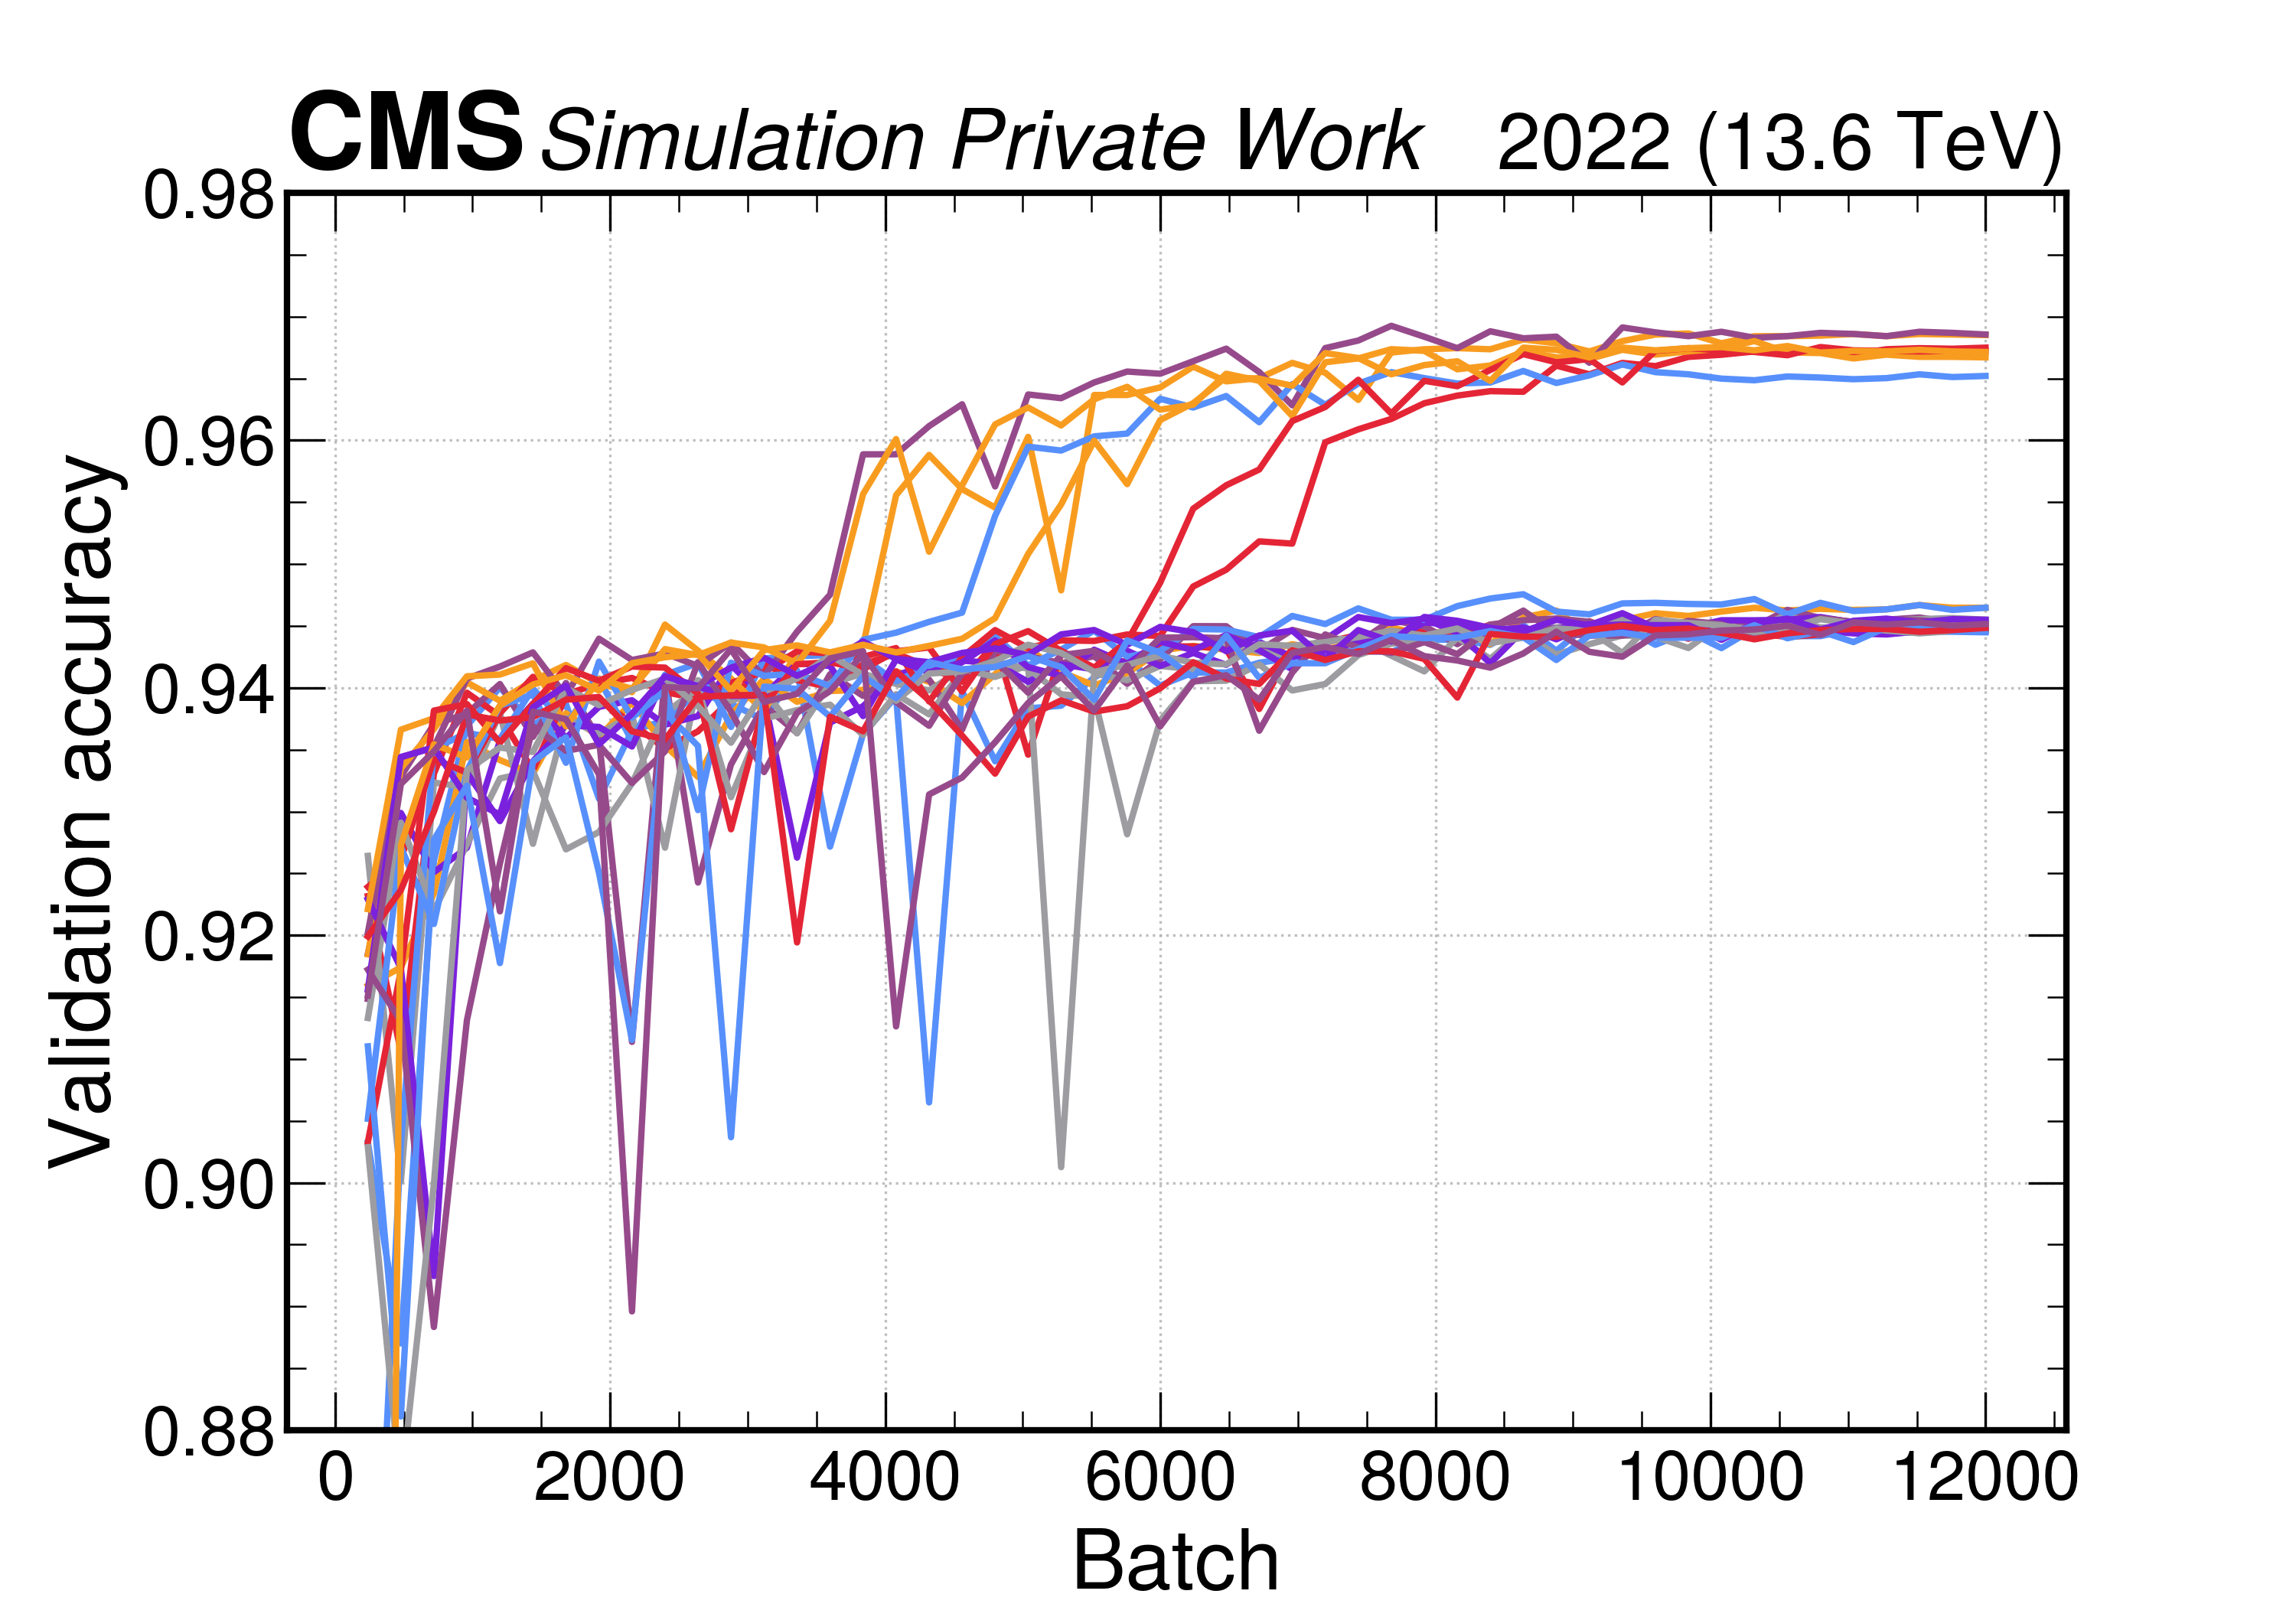
\includegraphics[scale=0.1]{Images/6.Improving/Variability Study/5 jets variability study.png}
    \caption{Variability on the training using 5 jets as inputs \pt reg and lite model parameters}
    \label{fig: 5j variability}
\end{figure}

With the lite model we are using the following hyperparmeters that we aim to modify:

\begin{table}[hbt]
\centering
\begin{tabular}{|p{5cm}|p{4cm}|p{5cm}|}
 \hline
 Hyperparemeters  & Lite model & Test for stabilization \\
 \hline
 Learning rate & 0.00659 & $5\times 10^{-3}$, $10^{-3}$, $5\times 10^{-4}$, $10^{-4}$ \\
 \hline
 Learning rate warmup cycles & 1 & 0\\
 \hline
  Learning rate cycles & 1 & 0\\
 \hline
 Batch size & 2048 / 1024 & 2048/1024 \\
 \hline
 Number of epochs & 50/300 & 50/300 \\
 \hline
\end{tabular}
\caption{Possible variations of the hyperparameters to stabilize the model}
\label{table: }
\end{table}

In figure \textbf{bla}, we show how the learning rate changes using these new parameters. We can see that instead of reaching the peak of the learning rate after a few epochs, it starts from the maximal value and linearly decreases. After several trainings, we concluded that the most stable configuration is given by the learning rate $10^{-4}$. As we can see in Figure \textbf{bla}, when using the new hyperparameters, taking the smallest learning rate and a batch size of 2048, we see that all of our trainings now cluster around 95.9-96.4\%, which gives a spread of 0.5\%. This variability is acceptable as even taking into account this variability we outperform the Run 2 pairing efficiency. When using a batch size of 1024, our trainings cluster around the same value but with a spread of 0.3\%. However, to use a batch size of 2048 allows us to have faster trainings, therefore, since the difference in the spread is not very significant, we decided to keep a batch size of 2048. 


Finally, we studied the difference in the efficiency when varying the number of epochs. In Figure \textbf{bla} we can see that is improved by around 0.4\% when using 300 epochs. In conclusion, after this study the most stable and efficient configuration is given by the parameters showed in Table \ref{table: stable model} .

\begin{table}[hbt]
\centering
\begin{tabular}{|c|c|}
 \hline
 Parameters  & Stable model  \\
 \hline
 Learning rate &  $10^{-4}$ \\
 \hline
 Learning rate warmup cycles &  0\\
 \hline
  Learning rate cycles & 0\\
 \hline
 Batch size & 2048 \\
 \hline
 Number of epochs & 300 \\
 \hline
\end{tabular}
\caption{Configuration for the Stable model}
\label{table: stable model}
\end{table}


We will stick to this configuration for our model in the following sections. As a last test to increase the performance of our model, we perform a grid search, thank to which we are able to tune some of our parameters. This will be presented in the following section.


\subsection{Grid search}
To increase the pairing efficiency, we performed a grid search in order to tune some of the parameters. 
To do so, we used the features of the Stable model and changed the hyperparameters presented in Table \ref{table: parameters for the grid search}. 
However, contrary to what is specified in Table \ref{table: stable model} for this grid search we will use 50 epochs given the limited resources at our disposal.
As can be seen in Table \ref{table: parameters for the grid search}, we give different possible values for the hyperparameters and then we perform several tests combining them differently.
In particular for the first 3, we need to choose between the ones specifies, whereas for the L2 Penalty we can continually (in log scale) choose a value between [1e-5 : 1e-3].
The final output of this search will be the combination of hyperparameters that give the best performance which are shown in Table \ref{table: grid search}.


\begin{table}[hbt]
   \centering
   \begin{tabular}{|c|c|}
    \hline
    Hidden dimension  &  \{32, 64, 96\}  \\
    \hline
   Number of encoder layers & \{5, 6, 7, 8\} \\
    \hline
    Number of branch embedding layers &  \{1, 2, 3, 4\}\\
    \hline
     Number of branch encoder layers & 4\\
    \hline
    Number of regression layers & 3 \\
    \hline
    Number of classification layers & 1 \\
    \hline
    Focal gamma & 0.0 \\
    \hline
    L2 Penalty & [1e-5 : 1e-3] \\
    \hline
   \end{tabular}
   \caption{Final hyperparameters determined by the grid search}
   \label{table: parameters for the grid search}
   \end{table}



\begin{table}[hbt]
\centering
\begin{tabular}{|c|c|}
 \hline
 Hidden dimension  &  96  \\
 \hline
Number of encoder layers & 5 \\
 \hline
 Number of branch embedding layers &  3\\
 \hline
  Number of branch encoder layers & 4\\
 \hline
 Number of regression layers & 3 \\
 \hline
 Number of classification layers & 1 \\
 \hline
 Focal gamma & 0.0 \\
 \hline
 L2 Penalty & $7.3\times 10^{-4}$ \\
 \hline
\end{tabular}
\caption{Final hyperparameters determined by the grid search}
\label{table: grid search}
\end{table}

By using these new hyperparameters our model has 5.1 M trainable parameters compared to 0.5 M in the Stable model. 
As can be seen in Figure \textbf{bla}, by using this new hyperparameters, with which we have a much larger model, 
we don't increase that much the performance compared to the Stable model performance. 
Hence, we decided to use the hyperparameters from the Stable Model. (takes longer)

%Do i mention other traiinngs done by Mathieu?

\newpage

\subsection{Introducing the kl}

As explained in section \ref{section: HH4b}, by measuring the di-Higgs production we are aiming to study 
the Higgs boson self coupling parameter $\lambda$. To do so, by measuring the cross-section of the di-Higgs production, 
we can obtain information about the parameter lambda $\lambda$ as we can parameterize it in terms of anomalous Higgs
boson couplings $\kappa_\lambda$, where $\kappa_\lambda$ is defined as follows:

\begin{equation}
    \kappa_\lambda=\frac{\lambda_{HHH}}{\lambda^{SM}_{HHH}}
\end{equation}

As can be seen in Figure \textbf{bla}, for different $\kappa_\lambda$ the kinematics 
of our process change, therefore it is important to train SPANet accordingly. 
To do so, we will use multiple signal samples with different values of $\kappa_\lambda 
\in \{-2.0, -1.0, 0.0, 0.5, 1.0, 1.5, 2.0, 2.45, 3.0, 3.5, 4.0, 5.0\}$

Present the kl efficiencies of the first trainings just evaluated on the diffrent 
kl (slide 9- $2024_04_18-HH4b-SPANet_pairing$)

Presen the trainings using kl (sl 11/12)

Comparison od the efficiency of these new trainings sl 15


IN the presentation

%At some point I think there was something weird and I can present some of the kinematical variables I plot compared ti the official dataset.


We also compare traiings with kl as inputs or not, and there we say ok, so they perform the same so since we can't hace that info from data we choose the trainng with no kl as input.

\subsubsection{Loose/ Tight selections}

Presen the new cuts, and the distributions for the new evebts

Efficiency plots usin gtraiings with loose and tight cuts.

And accordimg to mass sculpting much better the tight


\subsection{THE OPTIMAL CONFIG}
% jets as inputs, pt reg, lite and stable model, tight cuts, no kl as inout explicitely



Preent the traiining dataset and nb of events after selections